\documentclass[sigconf]{acmart}

\usepackage{booktabs}

% Draft metadata. Replace the visibly marked fields before submission.
\setcopyright{none}
\settopmatter{printacmref=false,printfolios=true}
\acmConference[Conference Name]{Conference Full Name}{Month Day--Day, 2026}{City, State, USA}
\acmBooktitle{Proceedings of the Conference Name}
\acmYear{2026}
\acmDOI{}
\acmISBN{}

% Auditable rendering of the 28 semantic keys in outputs/paper/numbers.json.
% Values are display-formatted only; their exact values, selectors, derivations,
% source paths, byte counts, and SHA-256 fingerprints remain in numbers.json.
\expandafter\def\csname TD@abstract.primary_tract_count\endcsname{99}
\expandafter\def\csname TD@abstract.scenario_count\endcsname{3}
\expandafter\def\csname TD@abstract.preset_count\endcsname{3}
\expandafter\def\csname TD@abstract.transfer_tract_count\endcsname{88}
\expandafter\def\csname TD@abstract.transfer_scored_count\endcsname{86}
\expandafter\def\csname TD@methods.tool_count\endcsname{11}
\expandafter\def\csname TD@methods.agent_iteration_bound\endcsname{15}
\expandafter\def\csname TD@methods.critic_revision_bound\endcsname{2}
\expandafter\def\csname TD@methods.sandbox_timeout_s\endcsname{60}
\expandafter\def\csname TD@methods.retry_bound\endcsname{3}
\expandafter\def\csname TD@alignment.working_epsg\endcsname{5070}
\expandafter\def\csname TD@alignment.primary_raster_resolution_m\endcsname{39.816}
\expandafter\def\csname TD@alignment.primary_sentinel_count\endcsname{0}
\expandafter\def\csname TD@results.primary_population\endcsname{420{,}264}
\expandafter\def\csname TD@results.primary_tract_count\endcsname{99}
\expandafter\def\csname TD@results.primary_scored_count\endcsname{98}
\expandafter\def\csname TD@results.transfer_population\endcsname{300{,}879}
\expandafter\def\csname TD@results.transfer_tract_count\endcsname{88}
\expandafter\def\csname TD@results.transfer_scored_count\endcsname{86}
\expandafter\def\csname TD@results.transfer_unscored_count\endcsname{2}
\expandafter\def\csname TD@results.transfer_facility_count\endcsname{206}
\expandafter\def\csname TD@results.transfer_raster_width\endcsname{2{,}195}
\expandafter\def\csname TD@results.transfer_raster_height\endcsname{2{,}252}
\expandafter\def\csname TD@results.transfer_raster_resolution_m\endcsname{29.992}
\expandafter\def\csname TD@robustness.fixture_runs_per_cell\endcsname{20}
\expandafter\def\csname TD@robustness.rate_count\endcsname{2}
\expandafter\def\csname TD@robustness.fault_kind_count\endcsname{5}
\expandafter\def\csname TD@limitations.county_count\endcsname{2}
\newcommand{\TD}[1]{%
  \ifcsname TD@#1\endcsname\csname TD@#1\endcsname%
  \else\textbf{[UNMAPPED: #1]}\fi%
}

\begin{document}

\title{Write, Run, Repair: A Self-Debugging GeoAI Agent for Equity-Centered Coastal Flood-Risk Analysis}

\author{Manoj Sankuru}
\affiliation{
  \institution{[Institution Name]}
  \department{[Department Name]}
  \city{[City]}
  \state{[State]}
  \country{[Country]}
}
\email{[email address]}

\author{Caroline Nyaboke}
\affiliation{
  \institution{Clemson University}
  \department{Nieri Department of Construction and Real Estate Development}
  \city{Clemson}
  \state{South Carolina}
  \country{USA}
}
\email{cmachuk@clemson.edu}

% The draft's unnamed additional-author entry is omitted until a name and
% affiliation are supplied; inventing author metadata would be misleading.

\author{Jason Lucas}
\affiliation{
  \institution{Clemson University}
  \department{Nieri Department of Construction and Real Estate Development}
  \city{Clemson}
  \state{South Carolina}
  \country{USA}
}
\email{[email address]}

\begin{abstract}
Multi-source flood-risk analysis is difficult to repeat because elevation,
boundaries, demographics, and facilities arrive with different spatial units,
coordinate systems, and failure modes. We present Write, Run, Repair, a GeoAI
agent that combines provenance-aware deterministic tools, bounded generated-code
execution, traceback-guided repair, and critic verification. The evaluation uses
\TD{abstract.primary_tract_count} Charleston County tracts, the same isolated
workflow in \TD{abstract.transfer_tract_count} Chatham County tracts, and
\TD{abstract.scenario_count} fixed water-level scenarios crossed with
\TD{abstract.preset_count} preference presets. The transfer retains all units
while scoring \TD{abstract.transfer_scored_count}. Results demonstrate
traceable county-relative prioritization and sensitivity to normative weights;
they do not claim hydrodynamic forecasting, route optimization, or autonomous
public-safety decisions.
\end{abstract}

\keywords{GeoAI, flood risk, social vulnerability, spatial alignment, provenance, responsible AI}

\maketitle

\section{Problem Statement}

Coastal emergency planning requires combining physical hazard, population, and
capacity evidence before local decisions can be discussed. This integration is
scientifically and operationally fragile: a plausible map can hide a CRS error,
a failed service can be mistaken for a zero, and a single composite score can
conceal value judgments. Flood disruption also disproportionately affects people
with fewer mobility and recovery resources \cite{yu2020,ermagun2024}. Our
primary target is Charleston County, South Carolina; Chatham County, Georgia is
an isolated transfer case that tests whether the same county-neutral workflow
survives a new data boundary.

We evaluate fixed water-level scenarios of 1.5, 3.0, and 5.0~m over USGS 3DEP
elevation. For cell elevation $z$ and scenario height $h$, the deliberately
simple bathtub model is $d=\max(0,h-z)$. The heights are scenario inputs, not
forecasts for named storms; the model omits hydraulic connectivity, waves,
attenuation, and arrival time. We use the following operational definitions:
\emph{hazard} is modeled depth and tract inundated fraction; \emph{exposure} is
population in wet block-group portions aggregated to tracts; \emph{vulnerability}
is a percentile index of poverty, age 65+, disability, no-vehicle households,
and limited English proficiency; and \emph{resilience} is the protective
percentile of hospitals, schools, fire stations, and community centers within a
5-km straight-line radius. Vulnerability follows the rank logic of the
CDC/ATSDR SVI but uses only those five available indicators \cite{cdc2022}.

\emph{Equity} means making the population and vulnerable population represented
in a fixed ten-tract priority set visible under each declared weighting, along
with units displaced when weights change. \emph{Optimality} is therefore narrow:
the priority set is the highest county-relative score under a named preset. It
is not a globally optimal shelter allocation, route, capacity plan, or
travel-time solution. This definition keeps the implemented decision support
auditable and prevents the current evidence from answering a larger question
than it measures.

\begin{figure*}[t]
  \centering
  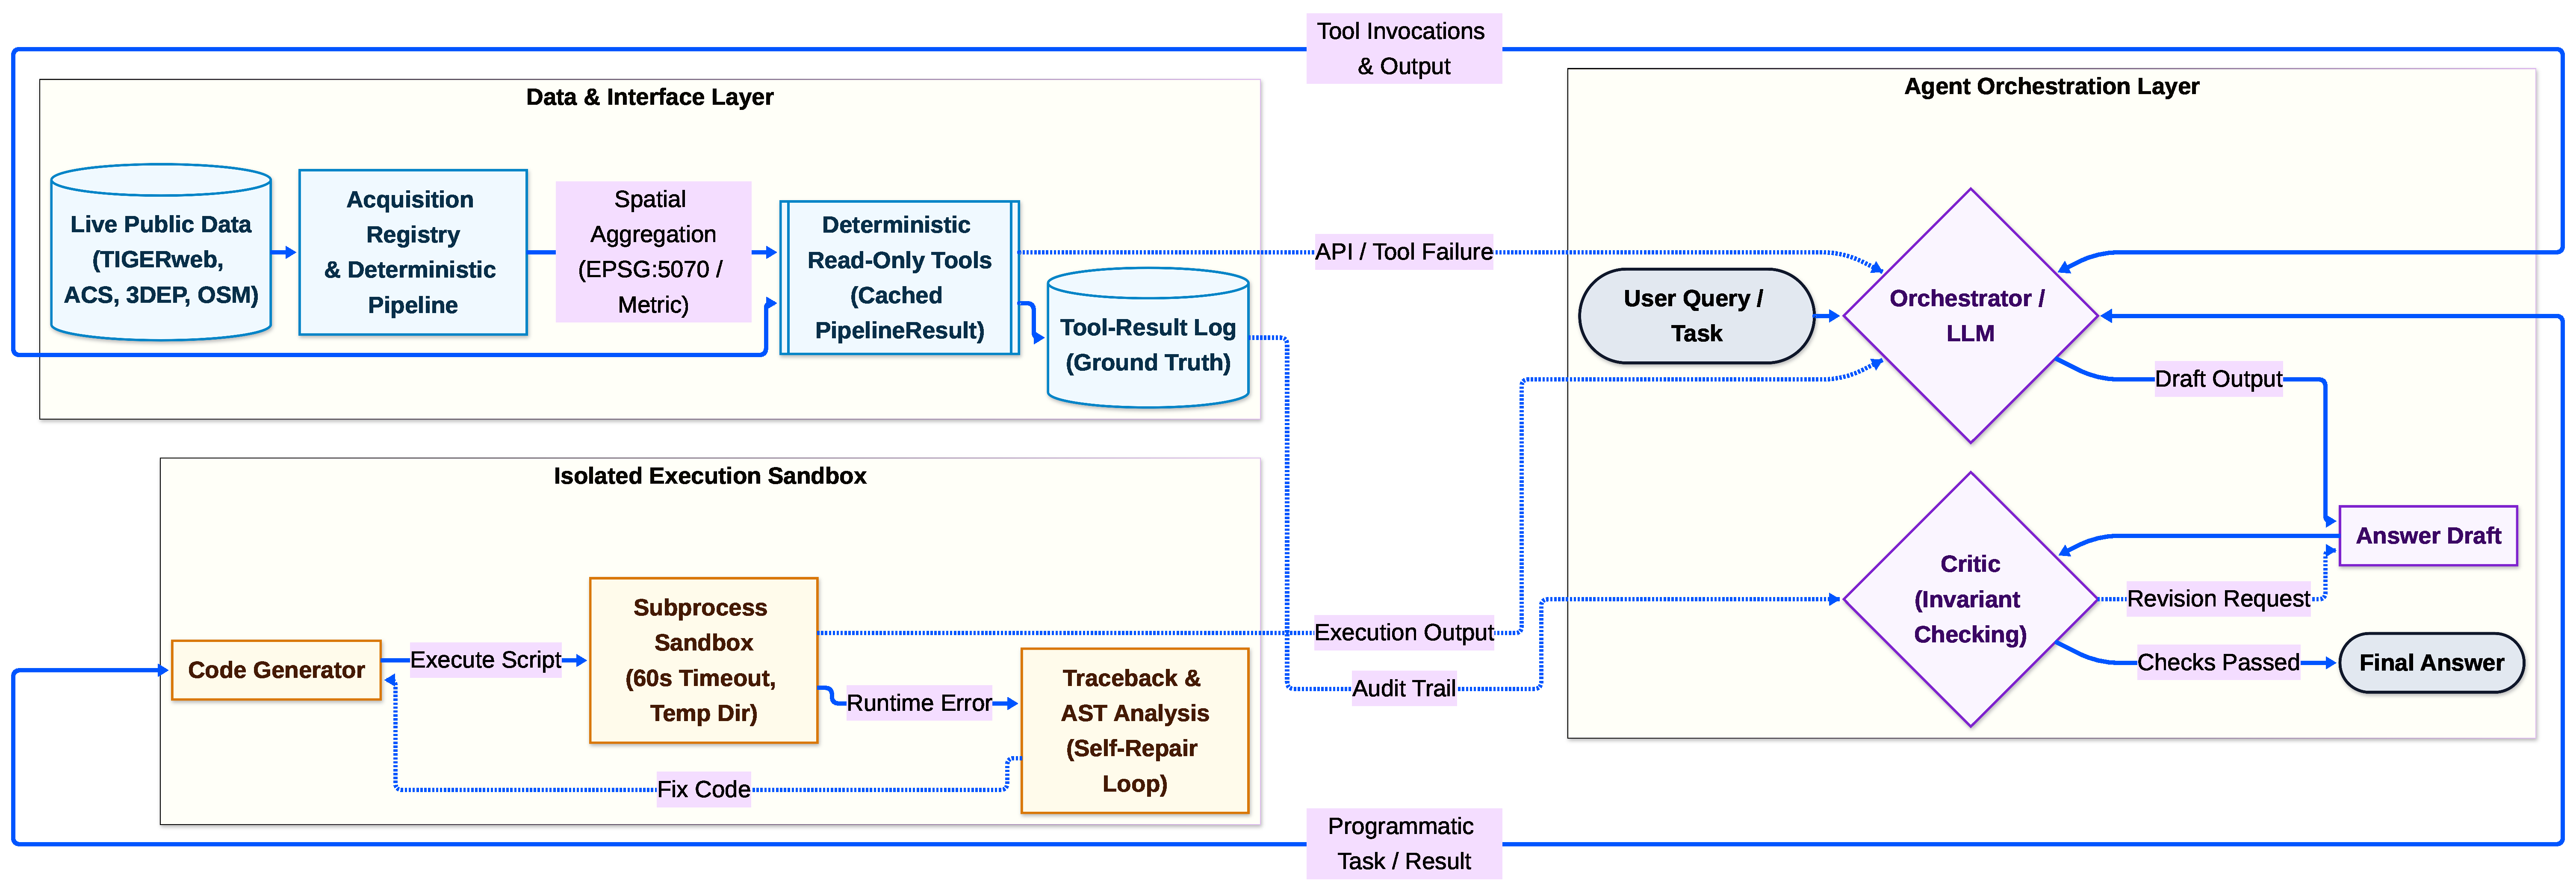
\includegraphics[width=\textwidth]{figs/architecture.pdf}
  \caption{WRR architecture decouples provenance-aware deterministic geospatial
  tools from the LLM orchestrator. Solid paths carry forward execution; dotted
  paths return tool evidence, failures, or revision requests through the
  traceback-guided code-repair and tool-log-guided critic-revision cycles.
  Geometry remains inside deterministic components, while summaries cross the
  model interface.}
  \Description{Dark three-layer diagram showing live public data, acquisition,
  deterministic tools, an orchestrating language model, tool-result logging,
  critic validation, generated code, bounded sandbox execution, traceback-guided
  code repair, revised drafts, and the final answer.}
  \label{fig:architecture}
\end{figure*}

\section{Agent Design}

\subsection{Architecture}

Figure~\ref{fig:architecture} separates the model-facing orchestration layer
from deterministic geospatial execution and exposes both bounded feedback
cycles and the summary-only model interface.

\subsection{Tool Orchestration}

An orchestrator selects from \TD{methods.tool_count} model-visible tools and may
use at most \TD{methods.agent_iteration_bound} agent iterations. The LLM selects operations
and interprets summaries, while registered tools own geometry, coordinates,
joins, raster operations, and evidence-bearing outputs.

\subsection{Data Acquisition}

The acquisition registry records URL, parameters, retrieval time, vintage,
license, declared/working CRS, feature count, and notes for Census TIGERweb
tracts and block groups, 2024 ACS tables, USGS 3DEP elevation, OpenStreetMap
facilities, and optional FEMA NFHL data. NFHL degraded in both evaluated areas;
the empty registered layer denotes unavailable regulatory-flood evidence, not
zero flood risk. No FEMA National Risk Index, HIFLD shelter, road-network, or
storm-specific surge raster is claimed as an input.

\subsection{Spatial Reasoning}

All metric operations use EPSG~\TD{alignment.working_epsg}. Geometry is repaired
and transformed through the alignment layer, GEOID joins are checked one to one,
and raster/vector coverage is verified before zonal statistics. The primary
3DEP grid has \TD{alignment.primary_raster_resolution_m}~m effective cells; the
alignment report recorded \TD{alignment.primary_sentinel_count} removed
sentinel values. Missing demographic indicators propagate to an unscored unit
rather than becoming a favorable zero. Risk retains the raw inundated fraction,
exposed population, vulnerability, and protective resilience components beside
their weighted percentile score, so a county-relative rank cannot be mistaken
for absolute danger.

\subsection{Error Recovery}

Unsupported analysis can produce GeoPandas/Rasterio code, which runs in a child
process with a \TD{methods.sandbox_timeout_s}-s timeout and scratch working
directory. A traceback is returned for repair; this resource boundary is not a
security sandbox. Separately, a critic checks the draft against logged tool
results and may request at most \TD{methods.critic_revision_bound} revisions.
Acquisition uses bounded retries of \TD{methods.retry_bound} attempts and
distinguishes transport failures, service-error bodies, truncated responses,
empty results, and CRS mismatches.

\section{Results and Analysis}

\subsection{Spatial Outputs}

\begin{table}[t]
  \caption{Validated population and tract coverage.}
  \label{tab:coverage}
  \centering
  \small
  \begin{tabular}{lrrr}
    \toprule
    Area & Population & Tracts & Scored \\
    \midrule
    Charleston & \TD{results.primary_population} &
      \TD{results.primary_tract_count} & \TD{results.primary_scored_count} \\
    Chatham & \TD{results.transfer_population} &
      \TD{results.transfer_tract_count} & \TD{results.transfer_scored_count} \\
    \bottomrule
  \end{tabular}
\end{table}

Table~\ref{tab:coverage} preserves the distinction between coverage and valid
scores. In Chatham, \TD{results.transfer_unscored_count} water/zero-universe
tracts remain present but are excluded from every ranking. Across both areas,
completed artifacts agree on scenario/preset membership, row counts, GEOID
domains, score/rank missingness, and top-ten membership; the primary alignment
also reports no unmatched joins or dropped/repaired geometries.

\begin{figure}[t]
  \centering
  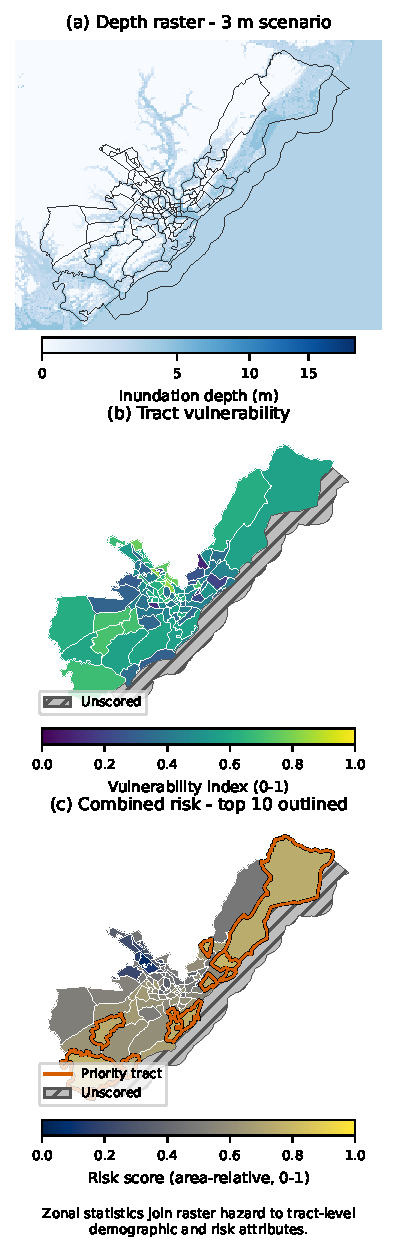
\includegraphics[width=\columnwidth]{figs/risk_surface.pdf}
  \caption{Charleston under the middle 3-m scenario and default equal-indicator
  preset: modeled inundation depth with tract boundaries, vulnerability, and
  combined county-relative risk. Heavy outlines mark the ten priority tracts;
  hatching denotes an explicitly unscored unit.}
  \Description{Three-panel Charleston map showing a blue inundation-depth raster,
  tract vulnerability, combined risk, and outlined priority tracts.}
  \label{fig:risk}
\end{figure}

Figure~\ref{fig:risk} makes the model boundary visible: the depth raster is
absolute scenario evidence, while vulnerability and combined risk are relative
within the county. The primary population total remains stable across scenarios;
what changes is modeled depth and the composition of the priority set.

The successful isolated transfer restored configuration and left the primary
snapshot unchanged. It registered \TD{results.transfer_facility_count}
facilities and produced a
\TD{results.transfer_raster_width}$\times$\TD{results.transfer_raster_height}
elevation grid at \TD{results.transfer_raster_resolution_m}~m effective
resolution.

\subsection{Sensitivity Analysis}

\begin{figure}[t]
  \centering
  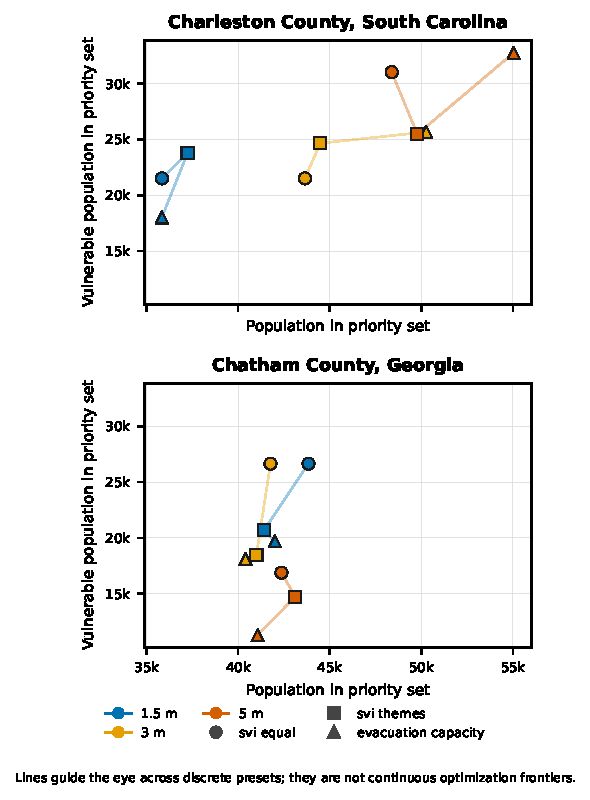
\includegraphics[width=\columnwidth]{figs/tradeoff.pdf}
  \caption{Priority-set sensitivity. Each panel separates one county; scenario
  color and preset marker identify each completed combination. Axes report total
  and vulnerable population in the fixed ten-tract set. Lines are visual guides
  within a county, not continuous optimization frontiers.}
  \Description{Two-panel scatter plot comparing population and vulnerable
  population in Charleston and Chatham priority sets across three water levels
  and three weighting presets.}
  \label{fig:tradeoff}
\end{figure}

Figure~\ref{fig:tradeoff} shows that normative assumptions matter. Changing the
indicator scheme or emphasizing evacuation capacity changes both the population
represented and which tracts are displaced; the direction is not uniform across
counties. Thus no preset dominates independently of the stated objective. The
figure is a sensitivity analysis over discrete, declared alternatives rather
than a claim that the system solved routing or shelter-location optimization.

\subsection{Failure Cases}

The transfer completed only after an initial 3DEP acquisition failure motivated
a global, county-neutral raster-size policy repair. The completed run is
therefore evidence of transfer after repair, not first-attempt or zero-change
portability. Optional NFHL retrieval also degraded in both areas and remained
explicitly labeled rather than being interpreted as zero flood exposure.

Retrieval robustness was measured offline with
\TD{robustness.fixture_runs_per_cell} seeded runs per cell, crossed over
\TD{robustness.rate_count} injection probabilities and
\TD{robustness.fault_kind_count} failure kinds. Increasing fault probability
reduced correctness in affected cells. Timeout and server-error cases exercise
retry recovery, while empty, truncated, and wrong-CRS responses demonstrate why
successful return is not equivalent to a correct dataset. The authoritative
artifact contains fixture rows only, so we do not generalize these rates to live
public services. Code-repair behavior and critic behavior are likewise not
quantified because no declared paper evaluation cohort exists.

\section{Social Impact and Reflection}

WRR can lower the cost of assembling an inspectable first-pass flood-risk
analysis and can help planners compare how explicit value choices affect the
communities brought forward for review. Its social benefit is transparency, not
automatic authority: component columns, provenance, missingness, displaced
units, and alternative presets make disagreement possible. Local officials and
community organizations should choose or reject weights, validate facilities,
and interpret results alongside lived experience.

The same automation creates risks. County-relative ranks can be mistaken for
absolute danger; ACS estimates and volunteered OSM facilities are incomplete;
missing data can disproportionately erase already undercounted communities; and
an authoritative-looking map can induce automation bias \cite{gevaert2021}.
Accordingly, the system refuses partial component scores, exposes degraded
sources, retains unscored units, and never converts its priority list into an
operational order. These safeguards improve auditability but do not establish
fairness or validate the chosen weights.

Several lessons were more important than model fluency. Provenance must be an
executable contract, spatial alignment must fail loudly, missingness must remain
visible, and retrieval repair must be separated from generated-code repair. The
transfer failure was useful precisely because it changed a global acquisition
policy rather than adding a county exception.

Limitations remain substantial. The bathtub surface is not hydrodynamic; the
facility-radius proxy has no roads, capacities, congestion, closures, or travel
times; only \TD{limitations.county_count} counties are evaluated; NFHL was
unavailable in both; robustness evidence is fixture-only; and agent behavior has
no declared evaluation cohort. The tool therefore supports exploratory
prioritization, not evacuation orders, shelter placement, or individual-level
decisions.

\section{Conclusion}

Write, Run, Repair demonstrates that a GeoAI agent can couple bounded tool
orchestration and repair with explicit spatial invariants and traceable evidence.
Across two coastal counties, three fixed-height scenarios, and three normative
presets, the implementation produces reproducible maps and discrete trade-off
comparisons while preserving degraded data and unscored units. The principal
contribution is not an optimal route plan, but an auditable workflow whose
assumptions and failure boundaries remain visible.

\begin{acks}
The authors thank [insert acknowledgment here].
\end{acks}

\bibliographystyle{ACM-Reference-Format}
\bibliography{refs}

\end{document}
